\section{Risorse}
Diciamo \textbf{Risorsa} un'entità astratta, necessaria ad un processo per svolgere il proprio lavoro. Quando la risorsa non è disponibile il processo dovrà attendere per utilizzarla.

\spacer
Alcune risorse che sono \textbf{condivisibili} e possono essere usate da più processi in parallelo. Mentre alcune risorse possono essere usate da un solo processo allo stesso tempo.

\spacer
Un'altra classificazione delle risorse separa quelle non consumabili (es. un core), mentre altre sono \textbf{consumabili} (es. un dispositivo a batteria).

\spacer
Utilizziamo il termine \textbf{preemption} per definire la rimozione forzata di una risorsa ad un processo.

\subsection{Grafico dei Processi}

\begin{figure}[H]
    \centering
    \begin{minipage}{0.45\textwidth}
        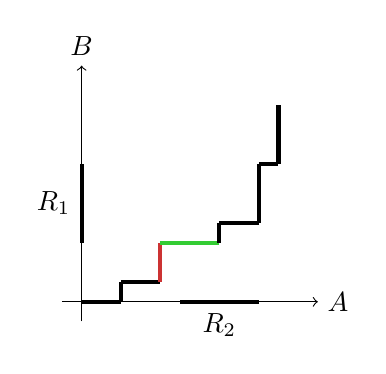
\begin{tikzpicture}[scale=2.5]
            % assi
            \draw[->] (-0.1,0) -- (1.2,0) node[right] {$A$};
            \draw[->] (0,-0.1) -- (0,1.2) node[above] {$B$};

            % grafico
            \draw[smooth, line width=1.5pt] (0, 0) -- (0.2, 0);
            \draw[smooth, line width=1.5pt] (0.2, 0) -- (0.2, 0.1);
            \draw[smooth, line width=1.5pt] (0.2, 0.1) -- (0.4, 0.1);
            \draw[smooth, line width=1.5pt, red!60!gray] (0.4, 0.1) -- (0.4, 0.3);
            \draw[smooth, line width=1.5pt, green!60!gray] (0.4, 0.3) -- (0.7, 0.3);
            \draw[smooth, line width=1.5pt] (0.7, 0.3) -- (0.7, 0.4);
            \draw[smooth, line width=1.5pt] (0.7, 0.4) -- (0.9, 0.4);
            \draw[smooth, line width=1.5pt] (0.9, 0.4) -- (0.9, 0.7);
            \draw[smooth, line width=1.5pt] (0.9, 0.7) -- (1, 0.7);
            \draw[smooth, line width=1.5pt] (1, 0.7) -- (1, 1);

            \draw[smooth, line width=1.5pt] (0, 0.3) -- (0, 0.5) node[left] {$R_1$};
            \draw[smooth, line width=1.5pt] (0, 0.5) -- (0, 0.7);
            \draw[smooth, line width=1.5pt] (0.5, 0) -- (0.7, 0) node[below] {$R_2$};
            \draw[smooth, line width=1.5pt] (0.7, 0) -- (0.9, 0);
        \end{tikzpicture}

        In questo caso i due processi A e B si alternano. Nel tratto rosso viene eseguito il processo B, mentre A è in attesa. Nel tratto verde accade l'opposto, il processo B che attende in favore di A.

        Le risorse $R_1$ e $R_2$ sono risorse non condivisibili, A usa $R_1$ e B $R_2$.

    \end{minipage}
    \hfill
    \begin{minipage}{0.45\textwidth}
        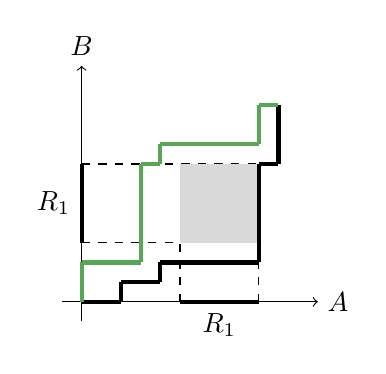
\begin{tikzpicture}[scale=2.5]
            % assi
            \draw[->] (-0.1,0) -- (1.2,0) node[right] {$A$};
            \draw[->] (0,-0.1) -- (0,1.2) node[above] {$B$};

            \draw[smooth, line width=1.5pt] (0, 0.3) -- (0, 0.5) node[left] {$R_1$};
            \draw[smooth, line width=1.5pt] (0, 0.5) -- (0, 0.7);
            \draw[smooth, line width=1.5pt] (0.5, 0) -- (0.7, 0) node[below] {$R_1$};
            \draw[smooth, line width=1.5pt] (0.7, 0) -- (0.9, 0);


            \draw[dashed] (0, 0.3) -- (0.5, 0.3);
            \draw[dashed] (0, 0.7) -- (0.9, 0.7);

            \draw[dashed] (0.5, 0) -- (0.5, 0.3);
            \draw[dashed] (0.9, 0) -- (0.9, 0.7);

            \draw[fill=gray!30, draw=none] (0.5,0.3) rectangle (0.9, 0.7);

            % grafico
            \draw[smooth, line width=1.5pt] (0, 0) -- (0.2, 0);
            \draw[smooth, line width=1.5pt] (0.2, 0) -- (0.2, 0.1);
            \draw[smooth, line width=1.5pt] (0.2, 0.1) -- (0.4, 0.1);
            \draw[smooth, line width=1.5pt] (0.4, 0.1) -- (0.4, 0.2);
            \draw[smooth, line width=1.5pt] (0.4, 0.2) -- (0.9, 0.2);
            \draw[smooth, line width=1.5pt] (0.9, 0.2) -- (0.9, 0.7);
            \draw[smooth, line width=1.5pt] (0.9, 0.7) -- (1, 0.7);
            \draw[smooth, line width=1.5pt] (1, 0.7) -- (1, 1);

            \draw[smooth, line width=1.5pt, green!30!gray] (0, 0) -- (0, 0.2);
            \draw[smooth, line width=1.5pt, green!30!gray] (0, 0.2) -- (0.3, 0.2);
            \draw[smooth, line width=1.5pt, green!30!gray] (0.3, 0.2) -- (0.3, 0.7);
            \draw[smooth, line width=1.5pt, green!30!gray] (0.3, 0.7) -- (0.4, 0.7);
            \draw[smooth, line width=1.5pt, green!30!gray] (0.4, 0.7) -- (0.4, 0.8);
            \draw[smooth, line width=1.5pt, green!30!gray] (0.4, 0.8) -- (0.9, 0.8);
            \draw[smooth, line width=1.5pt, green!30!gray] (0.9, 0.8) -- (0.9, 1);
            \draw[smooth, line width=1.5pt, green!30!gray] (0.9, 1) -- (1, 1);
        \end{tikzpicture}

        In questo caso invece i due processi devono condividere la stessa risorsa $R_1$, questo significa che il grafico non può mai entrare nell'area grigia.

        I due percorsi, nero e verde, sono entrambi validi per l'esecuzione dei due processi, entrambi passano al di fuori dell'area vietata.

    \end{minipage}
\end{figure}
